
\chapter{Przykłady wykorzystania promptów}
\label{cha:prompts}

Niekoniecznie jest potrzeba zaprezentowania każdego jednego wykorzystanego promptu, jednak te, które były kluczowe, powinny zostać udukomentowane, w tym w zakresie weryfikacji poprawności uzyskanego wyniku. Jeżeli prompt był punktem wyjścia, a grupa następnie rozwinęła jego wynik, to nadal należy ten fakt udokumentować.

\section{Przykład promptu AI}
W celu wstępnego rozeznania aplikacji podobnych do projektowanej wykonano następujący prompt w ChatGPT w wersji modelu GPT-4.1 mini. 

\begin{prompt}[htbp]
    \centering
    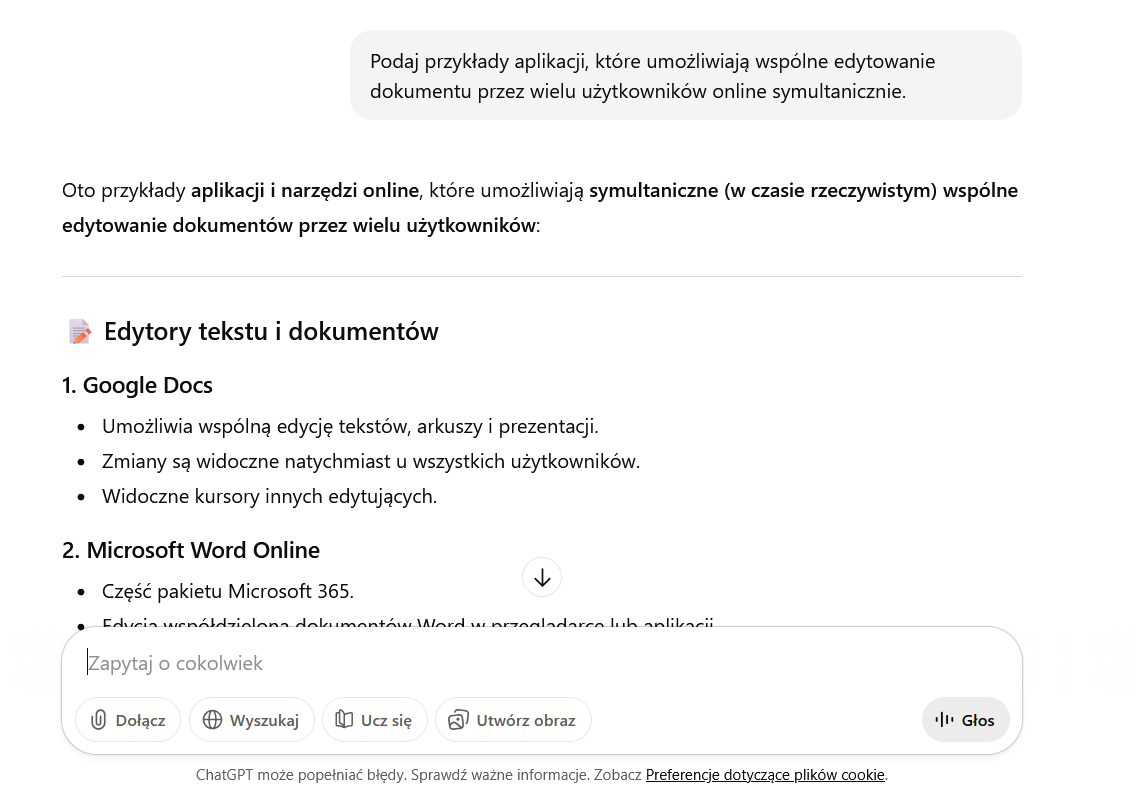
\includegraphics[width=\linewidth]{figures/prompts/chatGPT prompt.png}
    \promptcaption{Przykład promptu do wyszukania informacji}
    \label{prompt:info_searching}
\end{prompt}


Następnie sprawdzono proponowane przez model aplikacje i stwierdzono, że w rzeczywistości aplikacje przez niego proponowane zapewniają podobną funkcjonalność do projektowanej aplikacji. W dokumentacji rozszerzono opisy programów na bazie informacji dostarczonych przez narzędzie AI oraz dokumentacji tych programów.


\section{Przykład promptu AI z błędnym wynikiem, który należało poprawić}
Postanowiono wspomóc wygenerowanie diagramu przypadków użycia aplikacji za pomocą narzędzia AI. W tym celu napisano prompt, zawierajacy w sposób ogólny koncepcję aplikacji. Założono, że narzędzie AI samodzielnie zdefiniuje aktorów oraz konkretne przypadki użycia, jak i asocjacje pomiędzy aktorami a przypadkami użycia. Efekt tego zaprezentowano na prompcie \ref{prompt:use_case_polish}. 

\begin{prompt}[htbp]
    \centering
    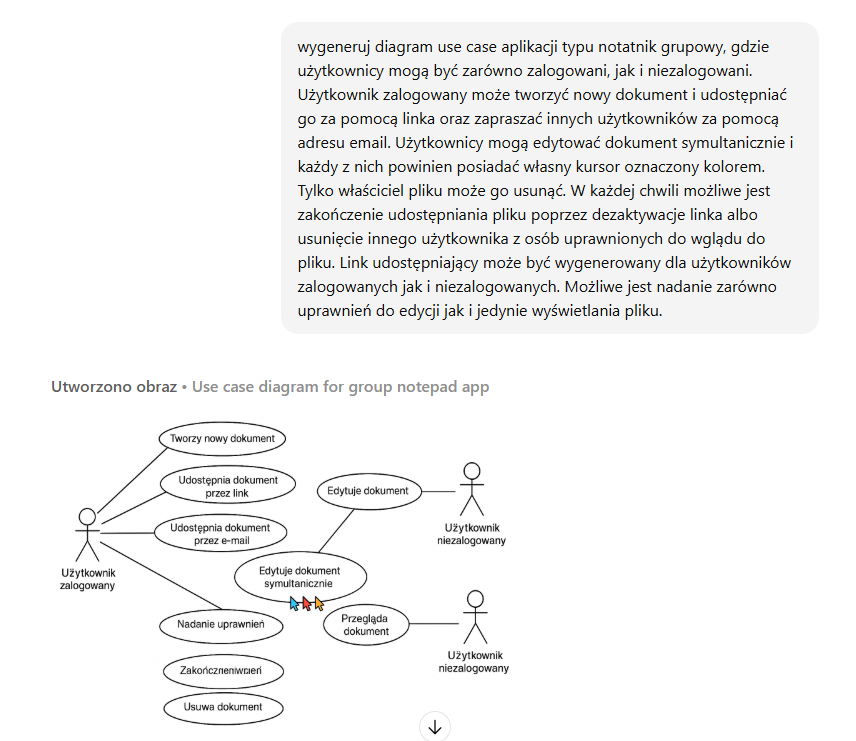
\includegraphics[width=\linewidth]{figures/prompts/use case prompt.png}
    \promptcaption{Początkowy prompt}
    \label{prompt:use_case_polish}
\end{prompt}

Łatwo można zauważyć, że narzędzie AI nie zinterpretowało polecenia w sposób oczekiwany. 
Wygenerowany diagram UML zawiera liczne błędy.
Wymaganie, aby każdy użytkownik posiadał własny kursor oznaczony innym kolorem nie zostało prawidłowo zaprezentowane jako przypadek użycia, ale w dość osobliwy sposób narysowane na diagramie, w sposób, który nie jest częścią notacji UML. Ponadto można zauważyć, że występują błędy ortograficzne i gramatyczne w wykorzystanym języku polskim. Również jeden z aktorów występuje na diagramie dwa razy. Ponadto niektóre przypadki użycia nie mają żadnej asocjacji z żadnym aktorem.

Wobec tego postanowiono przetłumaczyć prompt na język angielski i zobaczyć, czy polepszy to działanie modelu AI. Do przetłumaczenia prompta wykorzystano narzędzie deepL \cite{deepL}, treść wykorzystanego promptu zaprezentowano w \ref{prompt:translation}. Nie stwierdzono błędów językowych w wygenerowanym tłumaczeniu i ma ono treść zbieżną z poleceniem w języku polskim. Diagram przypadków użycia wygenerowany tym razem po angielsku zaprezentowano w  \ref{prompt:use_case_english}. Diagram ma większość takich samych błędów, jak wersja promptu wygenerowana w języku polskim, jedynie język angielski na diagramie w przeciwieństwie do polskiego wydaje się być poprawny gramatycznie. Wobec tego postanowiono poprosić o wygenerowanie wersji, którą będzie można łatwo edytować (być może należało zrobić tak na samym początku) za pomocą następującego promptu \ref{prompt:diagrams_net_use_case}. Diagram po wyrenderowaniu przez aplikację diagrams net zaprezentowano na Rysunku \ref{fig:diagrams_net_rendered}. Od razu można stwierdzić, że model generując diagram w tym formacie uzyskał dużo lepszy wynik niż wyjściowo. Aktorzy występują tylko jeden raz, każdy przypadek użycia posiada asocjacje (choć niepotrzebnie posiadają one strzałki) oraz sama zdefiniowanie przypadków użycia wydaje się tutaj dużo lepsze. Uznano że poza usunięciem strzałek z asocjacji nie ma potrzeby dalszej modyfikacji diagramu.


\begin{prompt}
    \centering
    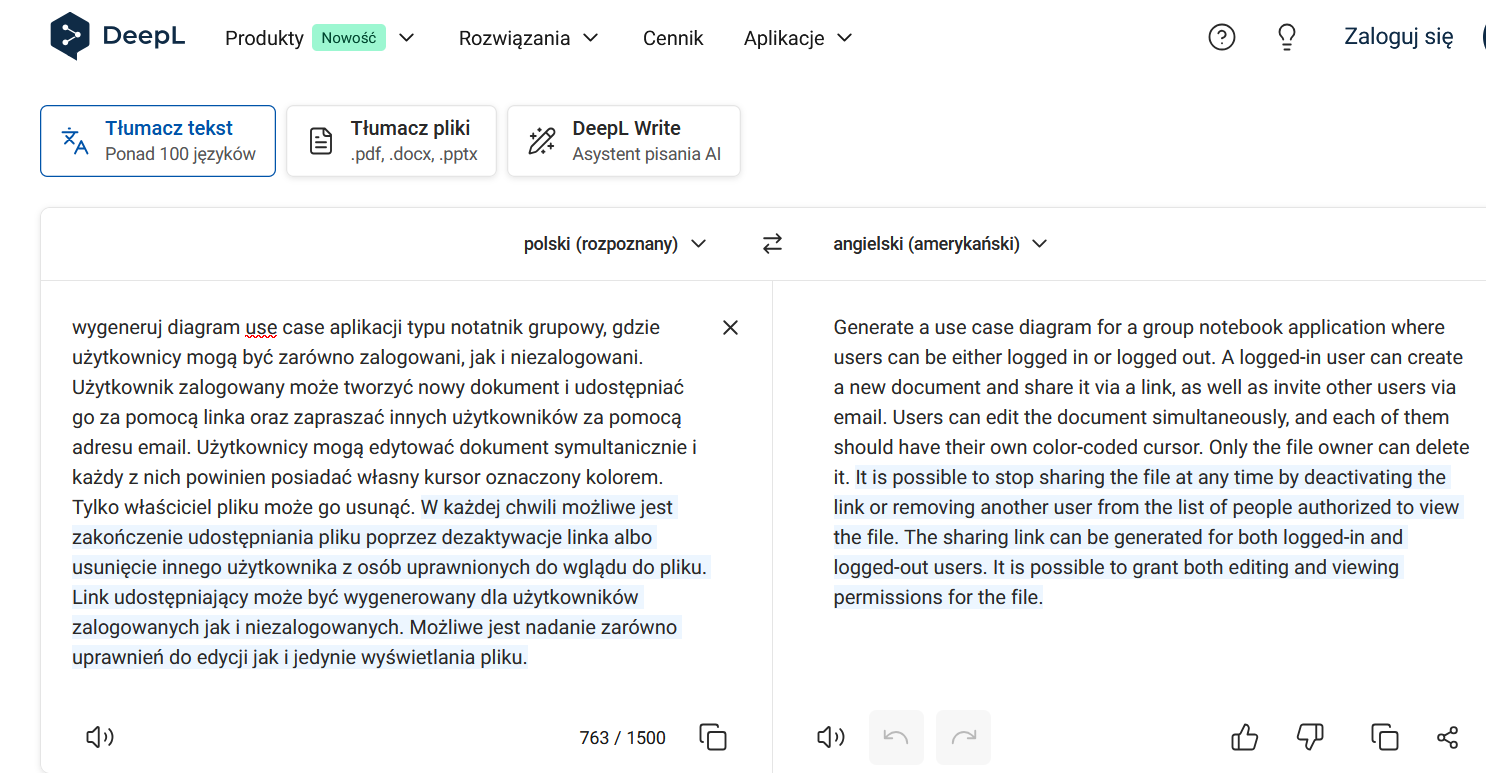
\includegraphics[width=\linewidth]{figures/prompts/prompt_translation.png}
    \promptcaption{Przykład tłumaczenia za pomocą generatywnej AI}
    \label{prompt:translation}
\end{prompt}



\begin{prompt}[htbp]
    \centering
    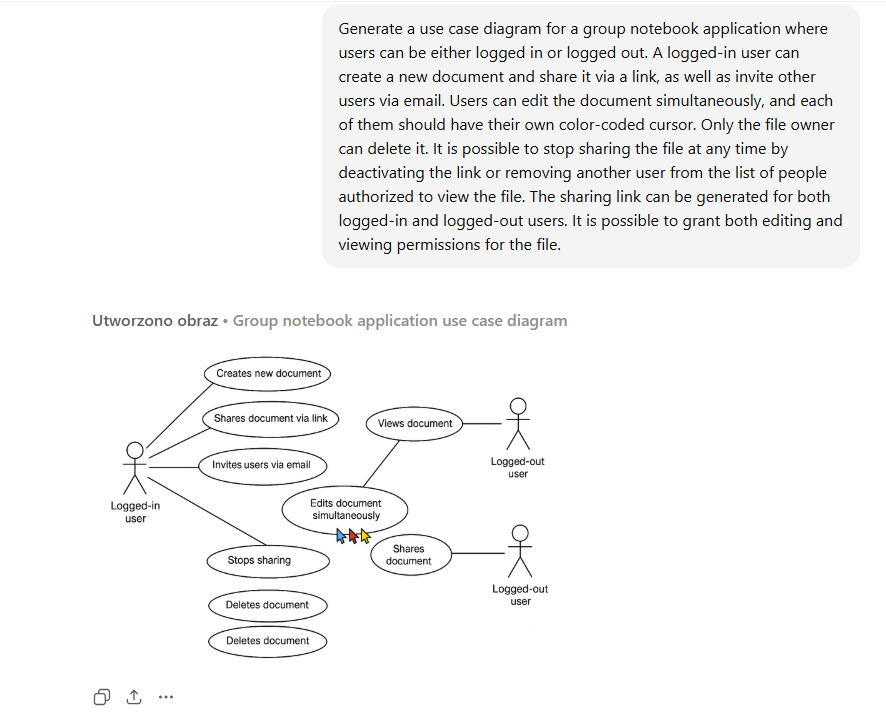
\includegraphics[width=\linewidth]{figures/prompts/use_case_english.png}
    \promptcaption{Kolejny prompt w języku angielskim}
    \label{prompt:use_case_english}
\end{prompt}

\begin{prompt}
    \centering
    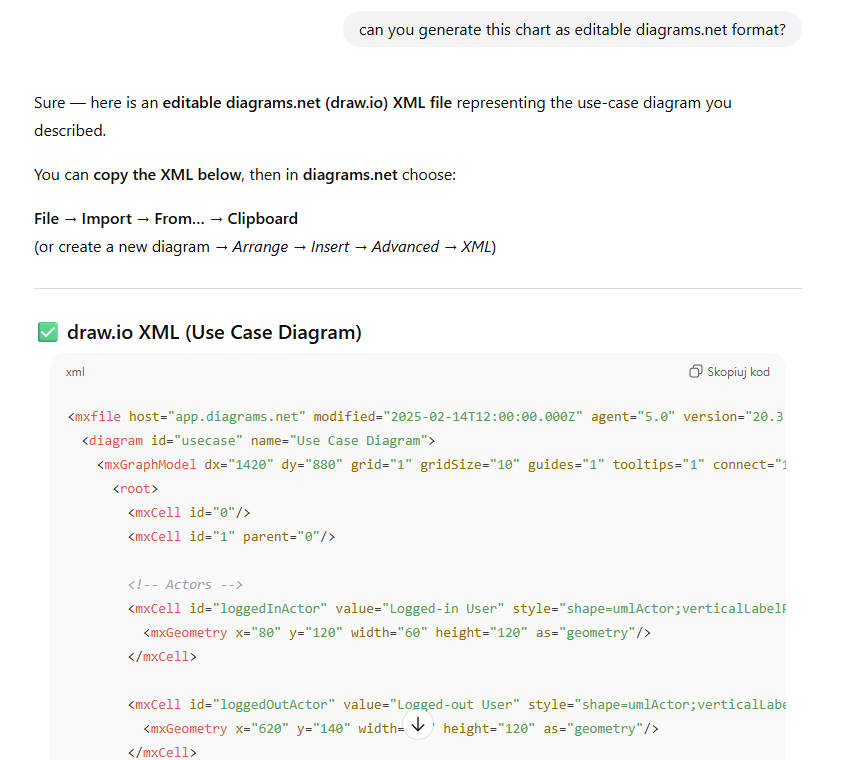
\includegraphics[width=\linewidth]{figures/prompts/diagrams_net_use_case.png}
    \promptcaption{Wygenerowanie diagramu przypadków użycia w postaci edytowalnej}
    \label{prompt:diagrams_net_use_case}
\end{prompt}

\begin{figure}
    \centering
    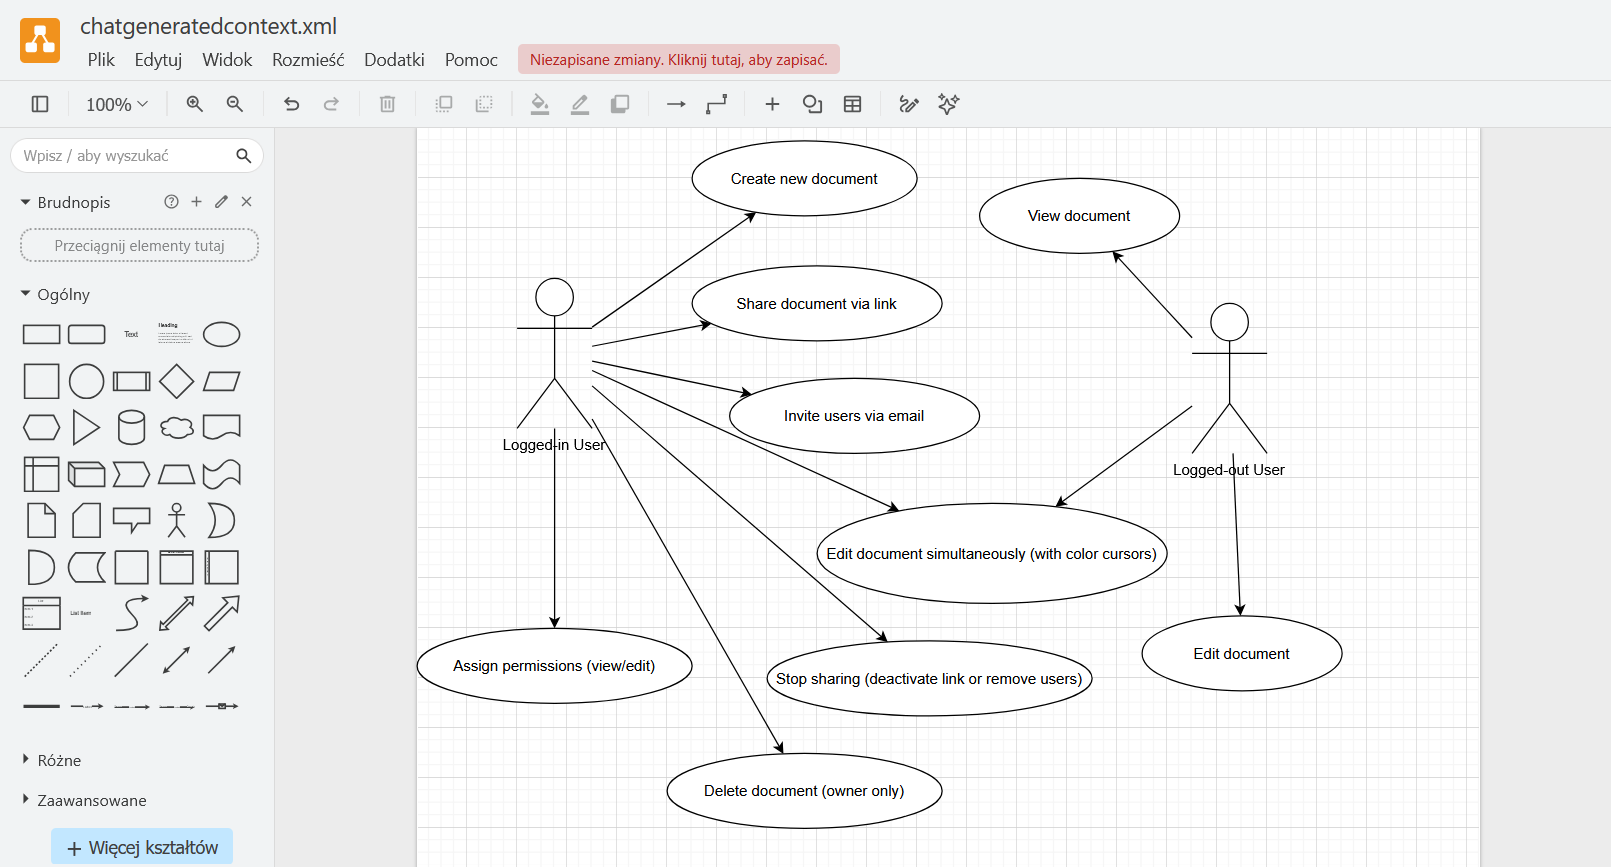
\includegraphics[width=\linewidth]{figures/prompts/diagrams_net_rendered.png}
    \caption{Wyrenderowany wynik działania promptu \ref{prompt:diagrams_net_use_case}}
    \label{fig:diagrams_net_rendered}
\end{figure}

